\chapter{The Boolean Satisfiability Problem}\label{chap:preliminaries}
\minitoc
In this thesis, our goal is to exploit the symmetry properties of SAT problems.
Before we get to the heart of the matter, we first introduce the Boolean satisfiability (SAT)  problem.
%This is a propositional formula representing constraints.
%A tool that aims to satisfy such formulas is called a SAT solver. 
%It answers $\sat$ when all constraints
%present in the formula can be satisfied and $\unsat$ otherwise.
\section{SAT basics}

The goal of SAT is to determine whether a propositional formula is satisfiable (i.e. all constraints can be satisfied)
or unsatisfiable (i.e. there is no way to satisfy all constraints at the same time).
The formula is constituted of \emph{Boolean} or \emph{propositional variables},
i.e. each variable has two possible values: true or false (noted respectively $\true$ or $\false$).
We call \emph{literal} a propositional variable or its negation.
For a given variable $x$, the positive literal is represented by $x$ and the negative one by $\neg x$.
Given a formula $\varphi$, we denote $\Vars_\varphi$ (respectively $\Lits_\varphi$) the set of variables (respectively literals) used in the formula (the index in $\Vars_\varphi$ and $\Lits_\varphi$ is usually omitted when
clear from context).
To build complex formulas, it is sufficient to use, $\neg, \lor$ and $\land$ which are respectively 
the negation, disjunction and conjunction operators. The remaining operators like, $\Rightarrow, \Leftrightarrow$ and
$\oplus, \cdots$ can be expressed using combinations of the basic ones.
For example, $a \Rightarrow b$, can be expressed as $ \neg a \lor b$.
Every binary operator adds a pair of parentheses to define explicitly the semantic of the formula.
In the absence of parentheses, the following priority order applies (from the highest to the lowest priority):
negation ($\neg$), conjunction ($\land$), disjunction ($\lor$).
An \emph{assignment}, noted $\alpha$, is defined as the function that assigns a value to each variable of $\varphi$:
 $$\alpha: \Vars \mapsto \{ \true, \false \}$$
 As usual, $\alpha$ is said \emph{total}, or \emph{complete}, when all elements of $\Vars$ have an image by
$\alpha$, otherwise it is \emph{partial}. By abuse of notation, an assignment is
often represented by the set of its true literals. For example, $\alpha = \{\neg x_1, x_3 \}$ means that $x_1$
is set to false and $x_3$ is set to true.
  The set of all (possibly partial) assignments of $\Vars$ is noted $\Assignments(\Vars)$.
A \emph{truth table} gives an evaluation of all possible assignments for a given formula.
\Cref{tab:truthtable} shows the evaluation of the negation ($\neg$), the conjunction ($\land$), and the disjunction ($\lor$) operators.
For convenience, the true value (\true) is also represented by $1$, and the false value (\false) is represented by $0$.
When a formula is always true, independently from the assignment, it is called a \emph{tautology}: $x \lor \neg x$ is 
an example of tautology.

\begin{table}[!htbp]
 \centering
 \begin{tabular}{cc|ccc}
  $x$ & $y$ & $\neg x$ & $x \lor y$ & $x \land y$ \\
  \toprule
  0 & 0 & 1 & 0 & 0 \\
  \midrule
  0 & 1 & 1 & 1 & 0 \\
  \midrule
  1 & 0 & 0 & 1 & 0 \\
  \midrule
  1 & 1 & 0 & 1 & 1 \\
  \bottomrule
 \end{tabular}
 \caption{Truth table of basic operators}
 \label{tab:truthtable}
\end{table}
%A formula is \textit{satisfiable} (noted $\sat$) if there exists at least one assignment that satisfies the formula
%Also, a formula is unsatisfiable ( noted $\unsat$) if it is not satisfiable.
A formula is said to be
\emph{satisfiable} (\sat) if there is at least one assignment that satisfies it;
otherwise the formula is \emph{unsatisfiable} (\unsat).
In order to compare different formulas, the concepts of logical equivalence and logical consequence
are defined in Definition~\ref{def:equiv} and Definition~\ref{def:logcons} respectively.

\vspace{1em}

\begin{definition}[Logical equivalence]\label{def:equiv}
 Two formulas $\varphi$ and $\psi$ are equivalent iff every assignment $\alpha$ that satisfies 
 formula $\varphi$  also satisfies the formula $\psi$ and vice versa. It is denoted by $\varphi \equiv \psi$.
\end{definition}


\begin{definition}[Logical consequence]\label{def:logcons}
 A formula $\psi$ is a \emph{logical consequence} of a formula $\varphi$ if each assignment that satisfies $\varphi$
  also satisfies $\psi$ and is denoted by $\varphi \models \psi$.
\end{definition}

\subsection{Normal forms}
In Boolean logic, there are some particular forms of formulas, called \emph{normal forms}.
 To introduce some of them, we first need to present the concepts of \emph{cube} and \emph{clause}.
\begin{definition}[Cube]
A cube $\gamma$ is a finite conjunction of literals represented equivalently by:
$$\gamma = \bigwedge_{i=1}^k l_i $$
\end{definition}

\begin{definition}[Clause]
A \emph{clause} $\omega$ is a finite disjunction of literals represented equivalently by:
$$\omega = \bigvee_{i=1}^k l_i \text{, or by the set of its literals } \omega = \{l_i\}_{i \in \llbracket 1,k \rrbracket}$$
\end{definition}

With respect to its size, a clause is said to be \emph{unary, binary, ternary,} $n$-ary if it contains respectively one, two, three, or $n$ literals.
%The clause form has a property called \emph{subsumption}. 
Clauses have the following property that can be exploited to simplify the formula.
When a clause $\omega_1$ is a subset of another clause $\omega_2$, noted $\omega_1 \subset \omega_2$,
we say that $\omega_{1}$ subsumes $\omega_{2}$.
 And any assignment that satisfies $\omega_1$ will also satisfy $\omega_2$. So, $\omega_2$ is \emph{redundant}
  with respect to  $\omega_{1}$ and can be removed from the formula.
 
 
\begin{definition}[Conjunctive Normal Form]
 The \emph{Conjunctive Normal Form} (CNF) of a formula is a finite conjunction of clauses. It can also be represented by
 $$\varphi = \bigwedge_{i=1}^k \omega_i \text{ (or by the set of its clauses } \varphi = \{\omega_i\}_{i \in \llbracket 1,k \rrbracket}\text{)}$$
\end{definition}

 \begin{definition}[Disjunctive normal form]
The \emph{Disjunctive normal form} (DNF) of a formula is finite disjunction of cubes.
I can be also represented by
$$\varphi = \bigvee_{i=1}^k \gamma_i$$
 \end{definition}


The following table is a summary of the laws that allow to transform any formula to
a normal form.

\begin{table}[!htbp]
 \centering
 \scriptsize
 \begin{tabular}{lllc}
  \multirow{2}{*}{Associativity laws} & $(x \lor y) \lor z \equiv x \lor (y \lor z)$\\
          & $(x \land y) \land z \equiv x \land (y \land z)$\\
  \hline              
  \multirow{2}{*}{Commutativity laws} & $x \lor y \equiv y \lor x$\\
          & $x \land y \equiv y \land x$\\
  \hline      
  \multirow{2}{*}{Identity laws} & $x \lor \false \equiv x$\\
           & $x \land \true \equiv x$\\
  \hline        
  \multirow{2}{*}{Domination laws} & $x \lor \true \equiv \true$\\
           &  $x \land \false \equiv \false$\\
  \hline        
  \multirow{2}{*}{Idempotent laws} & $x \lor x \equiv x$\\
               & $x \land x \equiv x$\\     
  \hline        
  \multirow{2}{*}{Distributive laws} & $x \lor (y \land z) \equiv (x \lor y) \land (x \lor z)$\\
           & $x \land (y \lor z) \equiv (x \land y) \lor (x \land z)$\\
 \hline        
 \multirow{2}{*}{Negation laws}  & $x \lor \neg x \equiv \true$\\
        & $x \land \neg x \equiv \false$\\
  \hline
   double negation law & $\neg (\neg x) \equiv x$ \\
  \hline
  \multirow{2}{*}{De Morgan’s laws} & $\neg x \lor \neg y \equiv \neg (x \land y)$\\
            &  $\neg x \land \neg y \equiv \neg (x \lor y)$\\
 \end{tabular}
 \caption{Set of laws of operators}
 \label{tab:laws}
\end{table}
Every formula can be transformed into a \textit{logically equivalent} normal form.
The Conjunctive normal form is the input form of state-of-the-art SAT solvers. Any propositional
formula can be transformed in CNF form with polynomial time\cite{Russell1994ArtiCI}. 
%Conversely, DNF form has
%an exponential memory complexity during the transformation\cite{darwiche2002knowledge}.
%Note that each cube in the problem in DNF form is a solution in the equivalent CNF formula.


%\hakan{Sharp SAT = transform CNF to DNF}
%A formula is said to be \emph{satisfiable} (\sat) if there is at least one assignment that satisfies it;
%otherwise the formula is \emph{unsatisfiable} (\unsat).
%\subsection{Satisfiability problem}
%A \emph{Boolean variable}, or \emph{propositional variable}, is a variable that
%has two possible values : true or false (noted respectively $\true$ or $\false$).
%A \emph{literal} $l$ is a propositional variable or its
%negation. For a given variable $x$, the positive literal is represented by $x$
%and the negative one by $\neg x$.
%
%A \emph{clause} $\omega$ is a finite disjunction of literals represented
%equivalently by $\omega = \bigvee_{i=1}^k l_i$ or the set of its literals
%$\omega = \{l_i\}_{i \in \llbracket 1,k \rrbracket}$. A clause with a single
%literal is called \emph{unit clause}.
%A clause is a \emph{tautology} if it is always true, a clause that contains a positive 
%and negative value of a clause for example.
%A \emph{conjunctive normal form (CNF) formula} $\varphi$ is a finite
%conjunction of clauses.  A CNF can be either noted $\varphi = \bigwedge_{i=1}^k
%\omega_i$ or $\varphi = \{\omega_i\}_{i \in \llbracket 1,k \rrbracket}$. We
%denote $\Vars_\varphi$ ($\Lits_\varphi$) the set of variables (literals) used in
%$\varphi$ (the index in $\Vars_\varphi$ and $\Lits_\varphi$ is usually omitted when
%clear from context).
%For a given formula $\varphi$, an \emph{assignment} of the variables of
%$\varphi$ is a function $\alpha: \Vars \mapsto \{ \true, \false \}$.  As usual, $\alpha$ is
%\emph{total}, or \emph{complete}, when all elements of $\Vars$ have an image by
%$\alpha$, otherwise it is \emph{partial}. By abuse of notation, an assignment is
%often represented by the set of its true literals.  The set of all (possibly
%partial) assignments of $\Vars$ is noted $\Assignments(\Vars)$.
%The assignment $\alpha$ \emph{satisfies} the clause $\omega$, denoted $\alpha
%\models \omega$, if $\alpha \cap \omega \neq \emptyset$. Similarly, the assignment
%$\alpha$ satisfies the propositional formula $\varphi$, denoted $\alpha \models
%\varphi$, if $\alpha$ satisfies all the clauses of $\varphi$. Note that a
%formula may be satisfied by a partial assignment. In this case, unassigned variable is called
%\emph{don’t care}.
%A formula is said to be
%\emph{satisfiable} (\sat) if there is at least one assignment that satisfies it;
%otherwise the formula is \emph{unsatisfiable} (\unsat).
\subsection{An NP-complete problem}
The SAT problem is the first NP-complete problem proven by Stephen Cook in 1971~\cite{cook1971complexity}.
NP-completeness means that a SAT problem can be solved with a non-deterministic Turing machine in polynomial time (NP) and is also NP-hard.
A problem is said to be NP-hard (non-deterministic polynomial-time hard) if 
any NP problem can be reduced to this problem in polynomial time.
If someone finds an algorithm that solves SAT in polynomial time, this answer 
one of the most important unsolved problems in theoretical computer science: the P versus NP problem,
 that is also one of the seven millennium prize problems~\cite{carlson2006millennium}.
 
 

\subsection{Some easy to solve forms}
Some particular instances of the SAT problem can be solved in polynomial time.

\paragraph{2-SAT~\cite{aspvall1979linear}.}

In this particular form, the given CNF formula contains only binary clauses.
Each clause is transformed into an implication and the conjunction of these form a directed graph called
binary implication graph.
For example, the clause $x \lor y$ will be transformed into $ \neg x \Rightarrow y$ and $\neg y \Rightarrow x$.
Then, a \emph{strong connected component} (SCC) is computed to determine the satisfiability of the formula.
If the same variable is present in both its positive and negative values in the same SCC then the formula is declared unsatisfiable,
otherwise a solution can be deduced and so the problem is satisfiable. 
This algorithm can be computed in linear time complexity.

%In this case, the formula that contains only binary clauses is transformed into a so called binary implication graph where each clause is transformed into an implication.


%Then, a \emph{strong connected component} (SCC) is computed to determine the satisfiability of the formula.
%If the same variable is present in both its positive and negative values in the same SCC then the formula is declared unsatisfiable,
%otherwise a solution can be deduced and so the problem is satisfiable. 
%This algorithm can be computed in linear time complexity.
%In this case, it suffices to create a graph in which each clause is transformed into implication. For example, the clause $x \lor y$ will be transformed into $ \neg x \Rightarrow y$ and $\neg y \Rightarrow x$.
%To determine the satisfiability of the formula, we need 
%\hakan{REDO}
% After computing \emph{strong connected component} on this graph, to be looking for the positive and negative forms of the same variable, in the same  strong connected component suffices 
%to determine the satisfiability of the formula.
% If it is the case, the formula is \unsat. Otherwise 
%a solution can be deduce and the problem is \sat. 

\paragraph{Horn SAT\cite{dowling1984linear}.} In this particular form, the given CNF formula contains only Horn clauses. 
There are three forms of Horn clauses: 
\begin{itemize}[topsep=0pt,itemsep=1pt]
\item \emph{strict Horn clause} that contains only one positive literal and at least one negative \\literal
\item \emph{positive Horn clause} that contains only one positive literal and no negative literals
\item \emph{negative Horn clause} that contains only negative literals.
\end{itemize}
To solve this particular form of formula, it suffices to  apply \emph{Boolean constraint propagation} (BCP) (or \emph{unit propagation}) explained in \cref{sec:dpll} until a fix point is reached.
Roughly speaking, it satisfies all unit clauses in cascade. At the end of the procedure, either an empty clause is deduced and the problem
is declared $\unsat$ or the fix point is reached and the formula is declared \sat.
 Like 2-SAT, this algorithm can also be computed in linear time complexity.
 
\paragraph{XOR SAT\cite{moore2011nature}.} In this particular form, each clause contains the xor ($\oplus$) operator rather than or ($\lor$).
This problem can be seen as a system of linear equations. Gaussian elimination is an algorithm that allows to solve this kind of
problem in polynomial time, more exactly in $O(n^3)$.

\subsection{Some related problems}
Different kinds of problems are related to SAT.
One of them is sharp-SAT (\#SAT)~\cite{valiant1979complexity}. Its purpose is to count the number of satisfiable assignments in a formula.
Another related problem is the \textit{maximum satisfiability problem} (MAX-SAT)~\cite{biere2009handbook}. In this case, the problem
is to find the maximum subset of clauses that can be satisfied for a formula. Different variants
of this problem exist. For example, some constraints must be satisfied (hard clauses) and MAX-SAT
is applied on the remaining clauses called \emph{soft} clauses.
The last related problem is quantified Boolean formula (QBF) where the quantifiers $\exists$ and
$\forall$ are present in the formula. For example, $\forall x\, \exists y\, \exists z \, (x \lor y) \land z$.
This particular form is a generalization of the SAT problem with PSPACE complexity~\cite{garey2002computers}.


\section{Solving a SAT problem}

\subsection{Algorithm}

Two kinds of algorithms exist to solve satisfiability problems.
First, \emph{incomplete} algorithms~\cite{kautz2009incomplete} which do not provide any guarantee that they will eventually report
either a satisfiable assignment or declare the formula unsatisfiable. This kind of algorithm is out of scope of this thesis. 
Second, the \emph{complete} algorithms, which provide a guarantee that if an assignment exists,
it will be found or declare that the formula is unsatisfiable.
This section describes different \emph{complete} algorithms to solve propositional formulas.

\subsubsection{A naive algorithm}
A naive approach to solve a SAT problem is to try all possible assignments.
For a propositional formula with $n$ variables, we have to verify, in the worse case, $2^n$ assignments.  
The algorithm first tries an assignment, for example all literals are set to false and then if
the formula is not satisfiable, it tries other assignments. 
This algorithm is finished when either a satisfiable assignment is found and so
the formula is declared $\sat$  or no assignment is satisfying the formula and so the formula is declared $\unsat$.
\Cref{fig:naive_algo} illustrates the search tree for a given problem with six variables.
The  formula presented in the figure has 6 clauses, with 2 ternary clauses and 4 binary clauses.
%It will be used as an example in different algorithm presented below. 
This formula is $\sat$, the assignment $\alpha_{11} = \{\neg x_1, \neg x_2, x_3, \neg x_4, x_5, \neg x_6 \}$ is a solution of the problem.
A naive algorithm might check 10 assignments before finding the solution. 
In the general case, due to the number of variables in problems, this algorithm will be intractable.


\begin{figure}[!htbp]
 \centering
 
\begin{minipage}[c]{0.6\linewidth}
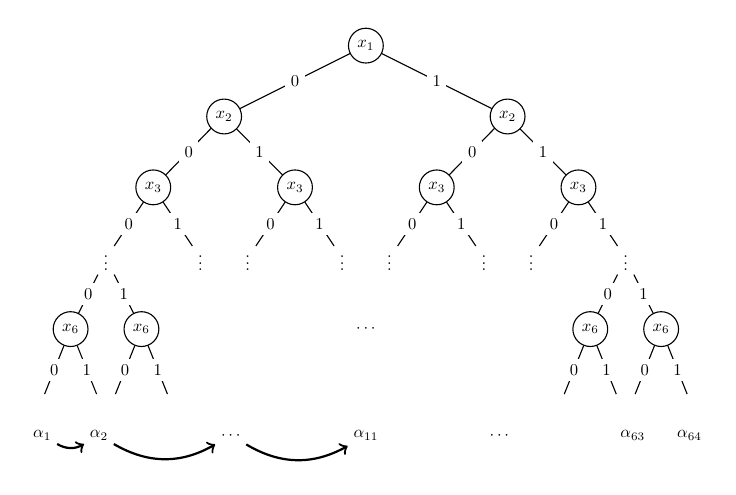
\begin{tikzpicture}[level/.style={sibling distance=60mm/#1},every node/.style={scale=0.6}, scale=0.6]
  \tikzstyle{trans}=[thick, ->, sloped]

\node [circle,draw] (x1) {$x_1$}
  child {node [circle,draw] (x2_1) {$x_2$}
    child {node [circle,draw] (x3_1) {$x_3$}
      child {node  (xn_1) {$\vdots$}
        child {node [circle,draw] (x6_1) {$x_6$}
        	child {node (x6_1f) {}
        	child[level distance=0.75cm] { node (a1) {$\alpha_1$} edge from parent[draw=none]}
        }
       		child {node (x6_1t) {}
       			child[level distance=0.75cm] { node (a2) {$\alpha_2$} edge from parent[draw=none]}
         }}
        child {node [circle,draw] (x6_2) {$x_6$}
        		child {node (x6_2f) {}}
        				child {node (x6_2t) {}
        	}
        }
      } 
      child {node (xn_2) {$\vdots$}}
    }
    child {node [circle,draw] (x3_2) {$x_3$}
      child {node (xn_3) {$\vdots$}}
      child {node (xn_4) {$\vdots$}}
    }
  }
  child {node [circle,draw] (x2_2) {$x_2$}
    child {node [circle,draw] (x3_3) {$x_3$}
      child {node (xn_5) {$\vdots$}}
      child {node (xn_6) {$\vdots$}}
    }
  child {node [circle,draw] (x3_4) {$x_3$}
    child {node (xn_7) {$\vdots$}}
    child {node (xn_8) {$\vdots$}
      child {node [circle,draw] (x6_3) {$x_6$}
      	       child {node (x6_3f) {}}
      	child {node (x6_3t) {}
        }}
      child {node [circle,draw] (x6_4) {$x_6$}
      	child {node (x6_4f) {}
        child[level distance=0.75cm] { node (an_1) {$\alpha_{63}$} edge from parent[draw=none]}
    	}
	    child {node (x6_4t) {}
    		child[level distance=0.75cm] { node (an) {$\alpha_{64}$} edge from parent[draw=none]}
      }}}
  }
};

\path (x6_2) -- (x6_3) node (x) [midway] {$\cdots$}
        child[level distance=2.25cm] { node (a_11) {$\alpha_{11}$} edge from parent[draw=none]};


\path (a2) -- (a_11) node (b1) [midway] {$\cdots$};
\path (a_11) -- (an_1) node (b2) [midway] {$\cdots$};

\draw[trans] (a1) to [bend right]  (a2);
\draw[trans] (a2) to [bend right]  (b1);
\draw[trans] (b1) to [bend right]  (a_11);

% to [bend right]  (b1) to [bend right]  (a_11);

\path (x1)   -- (x2_1) node [midway, fill=white] {$0$};
\path (x2_1) -- (x3_1) node [midway, fill=white] {$0$};
\path (x3_1) -- (xn_1) node [midway, fill=white] {$0$};
\path (xn_1) -- (x6_1) node [midway, fill=white] {$0$};
\path (x3_2) -- (xn_3) node [midway, fill=white] {$0$};
\path (x2_2) -- (x3_3) node [midway, fill=white] {$0$};
\path (x2_2) -- (x3_4) node [midway, fill=white] {$1$};
\path (x1)   -- (x2_2) node [midway, fill=white] {$1$};
\path (xn_1) -- (x6_2) node [midway, fill=white] {$1$};
\path (x3_1) -- (xn_2) node [midway, fill=white] {$1$};
\path (x2_1) -- (x3_2) node [midway, fill=white] {$1$};
\path (x3_2) -- (xn_4) node [midway, fill=white] {$1$};
\path (x3_3) -- (xn_5) node [midway, fill=white] {$0$};
\path (x3_3) -- (xn_6) node [midway, fill=white] {$1$};
\path (x3_4) -- (xn_7) node [midway, fill=white] {$0$};
\path (x3_4) -- (xn_8) node [midway, fill=white] {$1$};
\path (xn_8) -- (x6_3) node [midway, fill=white] {$0$};
\path (xn_8) -- (x6_4) node [midway, fill=white] {$1$};


\path (x6_1) -- (x6_1f) node [midway, fill=white] {$0$};
\path (x6_1) -- (x6_1t) node [midway, fill=white] {$1$};

\path (x6_2) -- (x6_2f) node [midway, fill=white] {$0$};
\path (x6_2) -- (x6_2t) node [midway, fill=white] {$1$};

\path (x6_3) -- (x6_3f) node [midway, fill=white] {$0$};
\path (x6_3) -- (x6_3t) node [midway, fill=white] {$1$};

\path (x6_4) -- (x6_4f) node [midway, fill=white] {$0$};
\path (x6_4) -- (x6_4t) node [midway, fill=white] {$1$};

\end{tikzpicture}
\end{minipage}
\begin{minipage}[c]{0.23\linewidth}
           \footnotesize
		\begin{itemize}
			\item[] $\omega_1 = \{x_1, x_2, x_3\}$ 
			\item[] $\omega_2 = \{x_4, x_5, x_6\}$
			\item[] $\omega_3 = \{\neg x_1, \neg x_5\}$
			\item[] $\omega_4 = \{\neg x_2, \neg x_4\}$
			\item[] $\omega_5 = \{\neg x_3, \neg x_4\}$
			\item[] $\omega_6 = \{\neg x_3, \neg x_6\}$
		\end{itemize}
\end{minipage}

 \caption{All possible assignments for a problem with 6 variables}
 \label{fig:naive_algo}
\end{figure}

\subsubsection{Davis Putnam Logemann Loveland algorithm (DPLL)}\label{sec:dpll}
One of the first, non-memory-intensive, algorithm developed to solve SAT problems is 
the Davis Putnam Logemann Loveland algorithm (DPLL)~\cite{dpll_62}. 
It explores a binary tree using depth first search, as shown in \Cref{algo:dpll}.
The construction of the tree  relies  on the unit propagation (\cref{algo:dpll:unit}) presented in detail in \Cref{algo:unitdpll} and on a \emph{decision} variable  that is chosen on \cref{algo:dpll:decision}.
Both values of this variable are checked, the true value on \cref{algo:dpll:pos} and the false value on \cref{algo:dpll:neg}.
When a leaf of the tree is inconsistent (i.e. a variable needs to be set to true and false at the same time), called a \textit{conflict} (\cref{algo:dpll:unsatbranch}), the opposite value of the decision is explored.
Recursively, when both values of a variable lead to a conflict,
the solver \emph{backtracks} one level (\emph{chronological backtracking}), i.e. tries the opposite value of 
the previous decision.
When the top of the tree is reached and a conflict occurs, it means that the formula cannot be satisfied and the 
solver reports $\unsat$ (\cref{algo:dpll:unsat}). However, if the formula is empty in any branch, 
this means that the current assignment satisfies the whole formula and the algorithm reports it on \cref{algo:dpll:sat1}
or \ref{algo:dpll:sat2}.

\clearpage

\begin{algorithm}[!htbp]
	\SetKwProg{Fn}{function}{}{}
	\SetKwFunction{DPLL}{DPLL}	
	\SetKwFunction{unitPropagation}{unitPropagation}
	\SetKwFunction{purePropagation}{purePropagation}
	\SetKwFunction{assignDecisionLiteral}{assignDecisionLiteral}

	
	\Fn{
		\DPLL{$\varphi$: CNF formula, $\alpha$ assignment}\\
		$\quad\quad$\textbf{returns} an assignment if $\varphi$ is \sat and $\unsat$ otherwise
	}
	{	
		$\varphi, \alpha \gets$ \unitPropagation{$\varphi, \alpha$}\;
	\label{algo:dpll:unit}
		\If{$\{\} \in \varphi$}{\Return \false \tcp*{Conflict}}	 \label{algo:dpll:unsatbranch}
		
		\If{$\varphi = \{\}$}{\Return $\alpha$ \tcp*{$\varphi$ is $\sat$}}
		
		$x \gets$ \assignDecisionLiteral{}\; \label{algo:dpll:decision}

		\If{$\alpha \gets$ \DPLL{$\varphi \cup \{x\}, \alpha $} \label{algo:dpll:pos}} 
		{
			\Return $\alpha$ 		\label{algo:dpll:sat1}
		}
		\If{ $\alpha \gets$ \DPLL{$\varphi \cup \{\neg x\}, \alpha $} \label{algo:dpll:neg}}
		{
			\Return $\alpha$ 		\label{algo:dpll:sat2}
		} 
	
		\Return \unsat \tcp*{$\varphi$ is $\unsat$}\label{algo:dpll:unsat}
	}
	\caption{The DPLL algorithm.}
	\label{algo:dpll}
	
\end{algorithm}

An important function in the DPLL algorithm is the Boolean constraint propagation (BCP) also called unit propagation 
(\Cref{algo:unitdpll})
This function set the values of unit clauses in order to satisfy them. It is applied until a fix point is reached: 
either there are no more unit clauses in the formula or an inconsistency is found.
The second case means that the current assignment cannot satisfy the formula and the
solver needs to backtrack to explore another branch.

\begin{algorithm}[!htbp]
	\SetKwProg{Fn}{function}{}{}
	\SetKwFunction{unitPropagation}{unitPropagation}
	\Fn{
		\unitPropagation{$\varphi$: CNF formula, $\alpha$ assignment}\\
		$\quad\quad$\textbf{returns}  CNF formula and assignment $\alpha$ 
	}
	{	
		\While{$\{l\} \in \varphi$ \textbf{and} $\{\} \notin \varphi$  }
		{
			\tcp{\small Remove all clauses containing $l$, all literals $\neg l$}
			$\varphi \gets \varphi\mid_{\,l}$\\
			$\alpha \gets \alpha \cup \{l\}$

		}
	\Return $\varphi, \alpha$
	}
	\caption{Unit propagation}
	\label{algo:unitdpll}
	
\end{algorithm}

When DPLL is executed on the formula of \Cref{fig:naive_algo}, after making decisions on literals
$\neg x_1$ and $\neg x_2$, unit propagation detects that $x_3$ must be assigned to true.
This propagation prevents to explore non-interesting assignments. Actually, when $x_3$ is set to false,
the clause $\omega_1$ cannot be satisfied and as it remains 3 variables and so $2^3$ possible assignments
(from $\alpha_1$ to $\alpha_8$). These assignments will never be checked.
The performance of the DPLL algorithm is highly impacted by the choice of decision variable.
\texttt{assignDecisionLiteral} is the procedure responsible of choosing it.
Its objective is to find a literal that will generate a maximum of unit propagations.
Intuitively, decision literals can be viewed as “guesses” and propagated literals can be viewed as “deductions”. 
Finding the optimal variable that will generate the maximum number of propagation is NP-Hard\cite{biere2009handbook}.
Different heuristics exists to choose the decision variable, some of them are presented in Section~\ref{sec:heuristics}.


%\input{algo/puredpll}
%Another idea introduced by DPLL was \emph{elimination of pure literals},
%a literal is said pure if it only appear on one sign (positive or negative) in the problem.
%These literals are set to true in the assignment.
%On consequence, all clauses that own these literals are satisfied and so can be removed.
%
\subsubsection{Conflict Driven Clause Learning (CDCL) algorithm}\label{sec:cdcl}
The principal weakness of the  DPLL algorithm is to discover the same inconsistencies several times
(principally due to chronological backtracking and absence of learning), leading to  unnecessary CPU usage.
Conflict Driven Clause Learning (CDCL) \cite{marques1999grasp} is a sound and complete algorithm
that overcomes this weakness.
\Cref{algo:cdcl} gives an overview of CDCL, like DPLL,  it walks on a binary search tree.
Initially, the  assignment is empty and the decision level that 
indicates the depth of the search tree, noted by $\mathit{dl}$, is set to zero.
The algorithm first applies unit propagation to the formula $\varphi$ for the  assignment $\alpha$ (\cref{alg:cdcl:unit}).
%Note that it is  the same procedure as the one used for DPLL.
An inconsistency or a \emph{conflict} at level zero indicates that the formula is unsatisfiable, and the algorithm
reports it (from \cref{alg:cdcl:unsat_start} to \cref{alg:cdcl:unsat_end}). When the conflict is occurring at a higher level,
 its reason is analyzed and a clause called \emph{conflict clause} is deduced (\cref{alg:cdcl:analyze}).
The work done in this procedure will be explained thereafter.
This clause is \emph{learnt} (\cref{alg:cdcl:learn}) (added to the formula). This clause is redundant with respect 
to the current formula, and so it does not change the satisfiability of $\varphi$.
 It also avoids encountering a conflict with the same
causes in the future. %This is the key difference with the DPLL algorithm.
The analysis is completed by the computation of a \emph{backjumps level}, the assignment and decision level are updated (\cref{alg:cdcl:backjump}).
 As the level can be much lower than the current level, this is called \emph{non-chronological backtracking} or \textit{backjump}.
Finally, if no conflict appears, the algorithm chooses a new decision literal 
(\cref{alg:cdcl:pick_start,alg:cdcl:pick_end}).
The above steps are repeated until the satisfiability status of the formula is determined.

\clearpage
\begin{algorithm}
	\SetKwProg{Fn}{function}{}{}
	\SetKwFunction{CDCL}{CDCL}
	\SetKwFunction{unitPropagation}{unitPropagation}
	\SetKwFunction{analyzeConflict}{analyzeConflict}
	\SetKwFunction{addLearntClause}{addLearntClause}
	\SetKwFunction{assignNewLiteral}{assignDecisionLiteral}
	\SetKwFunction{backjumpPolicy}{backjumpAndRestartPolicies}
	\SetKwFunction{ca}{currenttAssignment}
	\Fn{
		\CDCL{$\varphi$: CNF formula}\\
		$\quad\quad$\textbf{returns} $\true$ if $\varphi$ is \sat and $\false$ otherwise
	}
	{
		$dl \gets 0$ \tcp*{Current decision level}
		$\alpha \gets \emptyset$\;
		\While{not all variables are assigned}{
			$\varphi, \alpha \gets$ \unitPropagation{$\varphi|_\alpha, \alpha$}\;\label{alg:cdcl:unit}
			\If(\tcp*[f]{A conflict occurs}){ $\{\} \in \varphi$}
			{ 
				\If{dl = 0}{\label{alg:cdcl:unsat_start} 
					\Return \false \label{alg:cdcl:unsat_end} 
					\tcp*{$\varphi$ is $\unsat$}
				}
				$\omega \gets$ \analyzeConflict{}\;\label{alg:cdcl:analyze} 
				$dl \gets$ \backjumpPolicy{}\;\label{alg:cdcl:backjump} 
				$\varphi \gets \varphi \cup \{\omega$\} \; \label{alg:cdcl:learn}
				
			}
			\Else{
				$\alpha \gets \alpha\, \cup $ \assignNewLiteral{}\; \label{alg:cdcl:pick_start} 
				$dl \gets dl+1$\;\label{alg:cdcl:pick_end} 
			}
		}
		\Return \true
		\tcp*{$\varphi$ is $\sat$}
	}
	\caption{The CDCL algorithm.}
	\label{algo:cdcl}
	
\end{algorithm}



\subsection{Conflict Analysis}
A conflict is an inconsistency discovered by the solver, a situation that requires for a variable to be set 
simultaneously to the true and false. \Cref{fig:conflict} shows an example that leads to a conflict.
First, the solver chooses $\neg x_1$ as a decision (noted D ($\neg x_1$) in the figure) then, $\neg x_6$ and, then $\neg x_5$. This last one propagates $x_4$ (marked with P ($x_4$) in the figure),
which in turn propagates $x_2$ and $x_3$.
To satisfy $\omega_1$, $x_3$ needs to be set to $\true$, and  to satisfy $\omega_5$, 
it needs to be set to $\false$. As a variable cannot have both values, a conflict appears (noted C in the figure).

\begin{figure}[!htbp]
 \centering
  {\scriptsize
\newcommand{\ratioc}{0.195}
%\begin{minipage}[l]{\ratioc\linewidth}
%	\begin{itemize}
%		\item[] $\omega_1 = \{\cred{x_1}, x_2, x_3\}$ 
%		\item[] $\omega_2 = \{x_4, x_5, x_6\}$
%		\item[] $\cgreen{\omega_3} = \{\cgreen{\neg x_1}, \neg x_5\}$
%		\item[] $\omega_4 = \{\neg x_2, \neg x_4\}$
%		\item[] $\omega_5 = \{\neg x_3, \neg x_4\}$
%		\item[] $\omega_6 = \{\neg x_3, \neg x_6\}$
%	\end{itemize}
%\end{minipage}
\begin{minipage}[b]{\ratioc\linewidth}
	\begin{itemize}
	\item[] $\omega_1 = \{\cred{x_1}, x_2, x_3\}$ 
	\item[] $\omega_2 = \{x_4, x_5, \cred{x_6\}}$
	\item[] $\cgreen{\omega_3} = \{\cgreen{\neg x_1}, \neg x_5\}$
	\item[] $\omega_4 = \{\neg x_2, \neg x_4\}$
	\item[] $\omega_5 = \{\neg x_3, \neg x_4\}$
	\item[] $\cgreen{\omega_6} = \{\neg x_3, \cgreen{\neg x_6\}}$
\end{itemize}
\end{minipage}
\begin{minipage}[b]{\ratioc\linewidth}
		\begin{itemize}
		\item[] $\omega_1 = \{\cred{x_1}, x_2, x_3\}$ 
		\item[] $\omega_2 = \{\cprop{x_4}, \cred{x_5}, \cred{x_6\}}$
		\item[] $\cgreen{\omega_3} = \{\cgreen{\neg x_1}, \cgreen{\neg x_5\}}$
		\item[] $\omega_4 = \{\neg x_2, \neg x_4\}$
		\item[] $\omega_5 = \{\neg x_3, \neg x_4\}$
		\item[] $\cgreen{\omega_6} = \{\neg x_3, \cgreen{\neg x_6\}}$
	\end{itemize}
\end{minipage}
\begin{minipage}[b]{\ratioc\linewidth}
			\begin{itemize}
		\item[] $\omega_1 = \{\cred{x_1}, x_2, x_3\}$ 
		\item[] $\cgreen{\omega_2} = \{\cgreen{x_4}, \cred{x_5}, \cred{x_6\}}$
		\item[] $\cgreen{\omega_3} = \{\cgreen{\neg x_1}, \cgreen{\neg x_5\}}$
		\item[] $\omega_4 = \{\neg x_2, \cred{\neg x_4}\}$
		\item[] $\omega_5 = \{\neg x_3, \cred{\neg x_4}\}$
		\item[] $\cgreen{\omega_6} = \{\neg x_3, \cgreen{\neg x_6\}}$
	\end{itemize}
\end{minipage}
\begin{minipage}[b]{\ratioc\linewidth}
	\begin{itemize}
		\item[] $\omega_1 = \{\cred{x_1}, x_2, x_3\}$ 
		\item[] $\cgreen{\omega_2} = \{\cgreen{x_4}, \cred{x_5}, \cred{x_6\}}$
		\item[] $\cgreen{\omega_3} = \{\cgreen{\neg x_1}, \cgreen{\neg x_5\}}$
		\item[] $\omega_4 = \{\neg x_2, \cred{\neg x_4}\}$
		\item[] $\omega_5 = \{\neg x_3, \cred{\neg x_4}\}$
		\item[] $\cgreen{\omega_6} = \{\neg x_3, \cgreen{\neg x_6\}}$
	\end{itemize}
\end{minipage}
\begin{minipage}[b]{\ratioc\linewidth}
	\begin{itemize}
		\item[] $\omega_1 = \{\cred{x_1}, \cred{x_2}, \cblue{x_3}\}$ 
		\item[] $\cgreen{\omega_2} = \{\cgreen{x_4}, \cred{x_5}, \cred{x_6\}}$
		\item[] $\cgreen{\omega_3} = \{\cgreen{\neg x_1}, \cgreen{\neg x_5\}}$
		\item[] $\cgreen{\omega_4} = \{\cgreen{\neg x_2}, \cred{\neg x_4}\}$
		\item[] $\omega_5 = \{\cblue{\neg x_3}, \cred{\neg x_4}\}$
		\item[] $\cgreen{\omega_6} = \{\neg x_3, \cgreen{\neg x_6\}}$

	\end{itemize}
\end{minipage}
}


 \caption{Decisions/Propagations that leads to a  conflict}
 \label{fig:conflict}
\end{figure}

\clearpage

Applied another time, this serie of decisions would provoke the same propagation and lead to the same conflict. 
To escape this situation, one needs to analyze the situation and feed the algorithm with the information that prevents it to do the 
same mistake again. This is done by use of the so-called \emph{implication graph}.
%the solver needs to analyze the reason of the conflict with 
It represents the current state of the solver and records all dependencies between  variables. It is updated when a variable is assigned 
(on decision/propagation), or unassigned (on backjumping operation). The implication graph is a directed acyclic graph (DAG) in which a vertex represents an assigned variable labeled by $\mathit{l@dl(l)}$ where $l$ represents the assigned literal and $\mathit{dl(l)}$ represents the decision level of the literal $l$.
Root vertices that have no incoming edges represent decision literals. The remaining vertices represent
propagations.
Each incoming arc, labeled by a clause, represents the \emph{reason} of this propagation.
This clause must be \textit{assertive} (i.e. all  literals are false except one that is not yet assigned).
\Cref{fig:implication-graph} shows the implication graph of the previous example (\Cref{fig:conflict}).

\begin{figure}[!htbp]
 \centering
 
\begin{tikzpicture} % [level/.style={sibling distance=60mm/#1},every node/.style={scale=0.89}, scale=0.89]

	\tikzstyle{decision}=[draw,double,circle,fill=red!25,minimum size=45pt,inner sep=0pt]
	\tikzstyle{propagation}=[draw,circle,fill=white!25,minimum size=45pt,inner sep=0pt]
	
	\node[decision] (dx1) {$\neg x_1$@1};
	\node[decision] (dx6) at ($(dx1) + (0, -2)$) {$\neg x_6$@2};
	\node[decision, draw=orange!80] (dx5) at ($(dx6) + (0, -2)$) {$\neg x_5$@3};
	
	\node[propagation, draw=orange, line width=0.5mm] (px4) at ($(dx6) + (4, -1)$) {$x_4$@3};
	\node[propagation] (px3) at ($(dx5) + (12, 0)$) {$\neg x_3$@3};
	\node[propagation] (px2) at ($(dx6) + (8, 0)$) {$\neg x_2$@3};

	\node[propagation] (px33) at ($(dx5) + (12, 4)$) {$x_3$@3};


	\node[font=\bfseries] (reason) at (2,-6) {\textcolor{orange}{Reason Side}};
	\node[font=\bfseries] (reason) at (9,-6) {\textcolor{orange}{Conflict Side}};

	\path[->, draw, thick] (dx6) -- (px4) node [midway, fill=white] {$\omega_2$};
	\path[->, draw, thick] (dx5) -- (px4) node [midway, fill=white] {$\omega_2$};
	
	\path[->, draw, thick] (px4) -- (px3) node [midway, fill=white] {$\omega_5$};
	\path[->, draw, thick] (px4) -- (px2) node [midway, fill=white] {$\omega_4$};
	
	\path[->, draw, thick] (dx1) -- (px33) node [midway, fill=white] {$\omega_1$};
	\path[->, draw, thick] (px2) -- (px33) node [midway, fill=white] {$\omega_1$};
	\path[<->, draw, line width=1mm, color=blue!60] (px3) -- (px33);
	\path[line width=0.5mm, draw=orange] ($(px4.east) + (0.5, -2)$) -- ($(px4.east) + (0.5, 4)$)  
			   node [fill=white] {\textcolor{orange}{Cut 1}};
	
%	\path[line width=0.5mm, draw=orange!60] ($(px4.east) + (-3.5, -2)$) -- ($(px4.east) + (-3.5, 4)$)
%			   node [fill=white] {\textcolor{orange!70}{Cut 2}};
	
	% Legend
	
	\path[draw] (-1, -6.5) -- (13, -6.5);
	\node[decision, scale=0.3] (ld) at (0, -7) {};
	\node[align=left, text width=2.2cm] at (1.5, -7) {Decision};
	
	\node[propagation, scale=0.3] (lp) at (0, -7.7) {};
	\node[align=left, text width=2.2cm] at (1.5, -7.7) {Propagation};
	
	\node[scale=1.5] (lz) at (5, -7) {$\rightarrow$};
	\node[align=left, text width=2.2cm] at (6.5, -7) {Implication};
	
	\node[scale=1.5] (ld) at (5, -7.7) {\textcolor{blue!60}{$\leftrightarrow$}};
	\node[align=left, text width=2.2cm] at (6.5, -7.7) {Conflict};
	
	\node[propagation, draw=orange, line width=0.5mm, scale=0.3] (le) at (10, -7) {};
	\node[align=left, text width=2.2cm] at (11.5, -7) {UIP};
	
	\node[scale=2] (ld) at (10, -7.7) {\textcolor{orange}{\textendash}};
	\node[align=left, text width=2.2cm] at (11.5, -7.7) {Cut};
	\path[draw] (-1, -8.2) -- (13, -8.2);
\end{tikzpicture}

 \caption{Implication graph}
 \label{fig:implication-graph}
\end{figure}

The \texttt{analyzeConflict} procedure analyzes this graph to find the reason of the conflict. To do that, a search of a
\emph{unique implication point (UIP)} is performed. A UIP of the last decision level of the implication graph is a variable
which lies on every path from the decision to the conflict. Note that there might be many UIPs for a given decision level.
In such a case, UIPs are ordered according to the distance with the contradiction. The First UIP (FUIP) is the closest to
the conflict. It is well known that the FUIP provides the smallest set of assignment that is responsible for the
contradiction~\cite{zhang2001efficient}.
A UIP divides the implication graph in two sides with a \emph{cut}; the \emph{reason side} contains decision variables 
that are responsible of the contradiction and the \emph{conflict side} that contains the conflict. 
 A UIP is always in the reason side. \Cref{fig:implication-graph} depicts the cuts in the implication graph.
Once the reason side of a conflict is established, a conflict-driven clause (or simply conflict clause) is produced.
To build this clause, it suffices to negate the
literals that have an ongoing arc to the  cut that contains the UIP. In \Cref{fig:implication-graph}, the produced
learned clause will be $\omega_l = \{x_1, \neg x_4 \}$. Since the information of this clause is redundant regarding 
the original formula, it can be added without any  restriction. The conflict clause can be simplified
using the implication graph to reduce its size (by detecting redundancies~\cite{sorensson2009minimizing}).
 All learned clauses are stored in a clause database.
 
The \texttt{backjumpAndRestartPolicies} procedure is executed after producing the conflict clause.
All variables from the highest decision level to the current decision level are unassigned and so 
the current decision level and assignment are updated accordingly.
If a conflict implies only one level, the decision variable must be assigned 
to the opposite value at level 0. This means that this literal must be true without any decision.
Adding the conflict clause prunes the search space that obviously contains no solution.
This is the key point of the CDCL algorithm and the big difference with the DPLL algorithm.
 In our example on \Cref{fig:implication-graph}, the target decision level is 1 because the 
 highest decision level different that the current one constructed in the conflict clause is 1.
After backtracking, the conflict clause will be assertive and the FUIP is the only variable that has
not a value and so will be propagated in the next step of the algorithm. In our example, at the decision level 1 the
literal $x_1$ is set to the false value and the assertive conflict clause $\omega_l = \{x_1, \neg x_4 \}$ propagates $x_4$ to 
the false value .

 
 
\subsection{Heuristics}\label{sec:heuristics}

\paragraph{Decision heuristics.}
 The choice of the 
 decision variable has a huge impact on the 
overall solving time. It influences the number of propagations and so 
the depth of the search tree.
 The Variable State Independent Decaying Sum (VSIDS)~\cite{moskewicz2001chaff} measure is one of the most famous decision heuristics and is used
nowadays in almost all solvers; each variable has an activity and  is increased by a multiplicative factor 
when it participates to the resolution of a conflict.
%A solver has thousands conflicts during the solving and so activity of variables are very volatile.
Decision heuristics choose the unassigned variable with the highest activity.
%\hakan{AVOIR
%The idea behind this heuristic is to solve ‘hard’ part of problem at the top of the search tree.
%Hence, it is much more efficient when coupled with the restart heuristics}
%. 
Learning rate based branching (LRB~\cite{liang2016learning}) is the latest decision heuristic. It is a
generalization of VSIDS and its goal is to optimize the \emph{learning rate} (LR), defined as the ability to generate
learned clauses. The LRB of a variable is the weighted average (computed with \emph{exponential recency
weighted average} (ERWA))  value taken by its LR over the time. Unassigned variable with the highest LRB is chosen as a decision. 
%\hakan{A VOIR The idea behind this heuristics is to keep variables that used to generate learned clause in the search tree.}

\paragraph{Restarts heuristics.}
Another important mechanism is \emph{restart}. Basically, the solver abandons its current assignment and 
restarts from the top of the tree, while maintaining some information, like learned clauses, scores of variables, etc.
 The restart prevents the solver to get stuck in the same part of the search space (phenomenon known as heavy tailing~\cite{gomes1997heavy}).
Detecting this phenomenon has been widely treated in the literature~\cite{audemard2012refining,biere2008adaptive}.
These strategies are based on counting the number of conflicts or on the monitoring the current search’s depth.
Theoretically, a solver with restarts has a better result~\cite{huang2007effect} and is today
used in almost all state-of-the-art solvers.

\paragraph{Cleaning clause database.}
Storing  all learned clauses will end up with memory exhaustion and the cost of unit propagation will increase.
 So, the solver needs to develop a policy to eliminate some of them. These clauses are redundant with regards to the initial 
 problem, removing them will not affect the satisfiability of the formula.
  In the literature, different criteria exist.
 The size of the clause is one of them and is very often used by solvers. 
 A small clause has a better chance to participate to the unit propagation and so be useful for the solving.
 As a consequence, large clauses are removed.\\
\emph{Clause activity} is another criterion, a clause augments its activity when it participates to conflict analysis. 
Clauses with a lower activity that are not implied in the resolution of conflicts are removed.
 The last, often, used criterion is based on the Literal Block Distance (LBD) measure. It is a measure that computes the \emph{quality} of a clause.
It is based on the number of decision levels present in the clause. The more a clause has a high value of LBD and 
the weaker its quality is, and so it will be deleted from the clause database.
 
In current state-of-the-art solvers, multiple criteria are used and half of the learned clauses are removed during the clause database cleaning process.

\subsection{Preprocessing / Inprocessing}
In order to optimize solving time, some transformation can be applied to simplify the original formula.
This is done by \emph{preprocessing} the formula before the start of the solving.
When it is used during the solving (usually after a restart), it is called \emph{inprocessing}.
Simplification of the formula is made by removing clauses and/or variables.\\
\emph{Variable elimination} simplification is based on the \emph{resolution inference rule}~\cite{robinson1965machine}.
Consider the two clauses $\omega_1 = \{x_1, x_i, ..., x_j \}$ and $\omega_2 = \{\neg x_1, y_i, ..., y_j\}$.
The resolution inference rule allows to derive a clause $\omega_3 = \{x_i, ..., x_j, y_i, ..., y_j\}$ which is called
the \emph{resolvent} as it results from solving two clauses on the literal $x_1$ and $\neg x_1$.
%Moreover,  applying variable elimination until either an empty clause is derived (unsatisfiable formula) or 
%no more application of the resolution are possible (satisfiable formula). This is a complete algorithm to solve a SAT problem.
%Its major issue is to explicitly generate all resolvent and can be exponential in CNF size.
%Hence, the memory of the computer will be limiting factor.
\emph{Subsumption} aims at removing  clauses. Consider two clauses $\omega_1$ and $\omega_2$, such that
$\omega_1 \subset  \omega_2$, then $\omega_2$ can be safely removed from the original formula.
\emph{Self subsuming resolution} uses resolution rules and subsumption. at the same time,
the resolvent clause subsumes the original one. For example, $\omega_1 = \{x_1, \neg x_2\}$ and $\omega_2 = \{x_1, x_2, x_3\}$,
 then the resolvent clause will be $\omega_3 = \{x_1, x_3\}$ which subsumes $\omega_2$. This principle
is implemented in the \texttt{SatElite}~\cite{een2005effective} preprocessor engine and is used in almost all modern SAT solvers.

Other simplification techniques exist such as \emph{Gaussian elimination} which detects a sub formula in a XOR-SAT
form and solves it in a polynomial time~\cite{moore2011nature}. This technique can also be used in inprocessing~\cite{soos2010enhanced}. 
Some techniques exploit the structure of the original formula and add relevant clauses to speed up the resolution
time of the SAT solver. One of them uses the \textit{community structure} of the formula to find good clauses to add into.
A preprocessor engine doing that is \texttt{modprep}~\cite{ansotegui2015using}.
%The usage of symmetries also adds relevant clauses in the formula and will be detailed in the next chapter.
\subsection{Optimizing SAT solving}
With the emergence of multi-core architectures and the increasing power of computers, one way to optimize the solving
of a SAT problem is the exploitation of these cores. %Actually, SAT problems are a good candidate for parallelism.
\emph{Portfolio}, first introduced in \emph{ManySAT}~\cite{hamadi2008manysat}, is a technique that launches several SAT solvers in parallel with different heuristics (decisions, restarts, ...) that 
communicates or not between them. When one of them finds a solution or finds that none exists, the overall computation is finished.
Another technique to develop a parallel SAT solver is called \emph{divide and conquer}. In this technique,
the search space is divided  dynamically and submitted to different solvers that cooperate to find a solution.
This is used in different solvers like, for example~\cite{chu2008pminisat, lewis2007multithreaded}.
 Some specific techniques like load balancing and work stealing is applied to avoid a solver to be idle.
A recent framework \emph{PaInleSS} (a Framework for Parallel SAT Solving) can be used to easily create a new parallel 
SAT solver with different heuristics~\cite{le2017painless}~\cite{le2019modular}. 
Another way to optimize the solving time of SAT solvers is the exploitation of symmetries. The rest of this manuscript will 
detail how this allows to improve the performance of SAT solvers in the presence of symmetries in the original formula.
%Authors of this framework win the parallel tracks of SAT competition \footnote{\url{http://www.satcompetition.org/}} in 2018.
%\begin{center}
%\begin{tikzpicture}
%\begin{scope}[blend group = soft light]
%\fill[red!30!white]   ( 90:1.2) circle (2);
%\fill[green!30!white] (210:1.2) circle (2);
%\fill[blue!30!white]  (330:1.2) circle (2);
%\end{scope}
%\node at ( 90:2)    {$x$};
%\node at ( 210:2)   {$y$};
%\node at ( 330:2)   {$z$};
%\node (c) {$x \land y \land z$};
%
%\node at ($ (c) + (-1.2, .7)$)   {$x \land y$};
%\node at ($ (c) + (+1.2, .7)$)   {$x \land z$};
%\node at ($ (c) + (0, -1.3)$)   {$y \land z$};
%\end{tikzpicture}
%\end{center}